\section*{سنتزکردن کدها}

پس از این که به کمک دستورات نوشته‌شده با اسمبلی 
\lr{ARM}
 و کد پایتون ذکرشده، 
\lr{ROM}ای 
که در قسمت‌های قبل توضیح‌داده‌شد را پرکردیم؛ مجموعه کدهای وریلاگمان کامل خواهدشد و حال باید این کدها را سنتزکنیم.

برای سنتز کدهای وریلاگ از نرم افزار
\lr{Quartus}
 محصول شرکت
\lr{Altera}
   استفاده‌کردیم و برای این کار در کوارتوس یک پروژه ساخته و تمامی فایل‌هایی که می‌خواهیم سنتزکنیم (تقریبا تمامی فایل‌ها به جز تست‌بنچ‌ها) را به آن پروژه اضافه‌نمودیم. 

سپس با چندین بار تلاش برای سنتز کدها ، اشکالات موجود و بخش‌های غیرِ سنتزپذیر کد را از آن حذف‌کردیم و با قطعه کدهای سنتزپذیر جایگزین‌کردیم تا در نهایت سنتز ماژول اصلی یعنی ماژول
\lr{top} 
 که در اصل مربوط به
\lr{Integration} 
  تمامی مواردی بود که پیاده‌سازی کرده‌ایم، انجام‌شد.

برای راحت‌ترشدن اجرا و تست و
\lr{import }کردن 
 فایل‌های سنتزشده به نرم‌افزار مادل‌سیم، از یک اسکریپت استفاده‌کردیم که با گرفتن ورودی، خود به خود نرم‌افزار مادل‌سیم را بازکرده و شبیه‌سازی را انجام‌داده و نتیجه را به ما ارائه می‌دهد. این اسکریپت سبب شد که سرعت تست کردن کدها و نتایج بسیار بالا رود و بتوانیم سریع‌تر مشکلات کدها را یافته و آن ها را برطرف کنیم.

در نهایت پس از رفع اشکالات کد مذکور، بالاخره خروجی تولیدشده توسط کد با خروجی مورد انتظار ما مشابه‌شد که شکل آن را در شکل
\ref{fig:result}
 می‌کنید.

\begin{figure}[H]
	\centering
	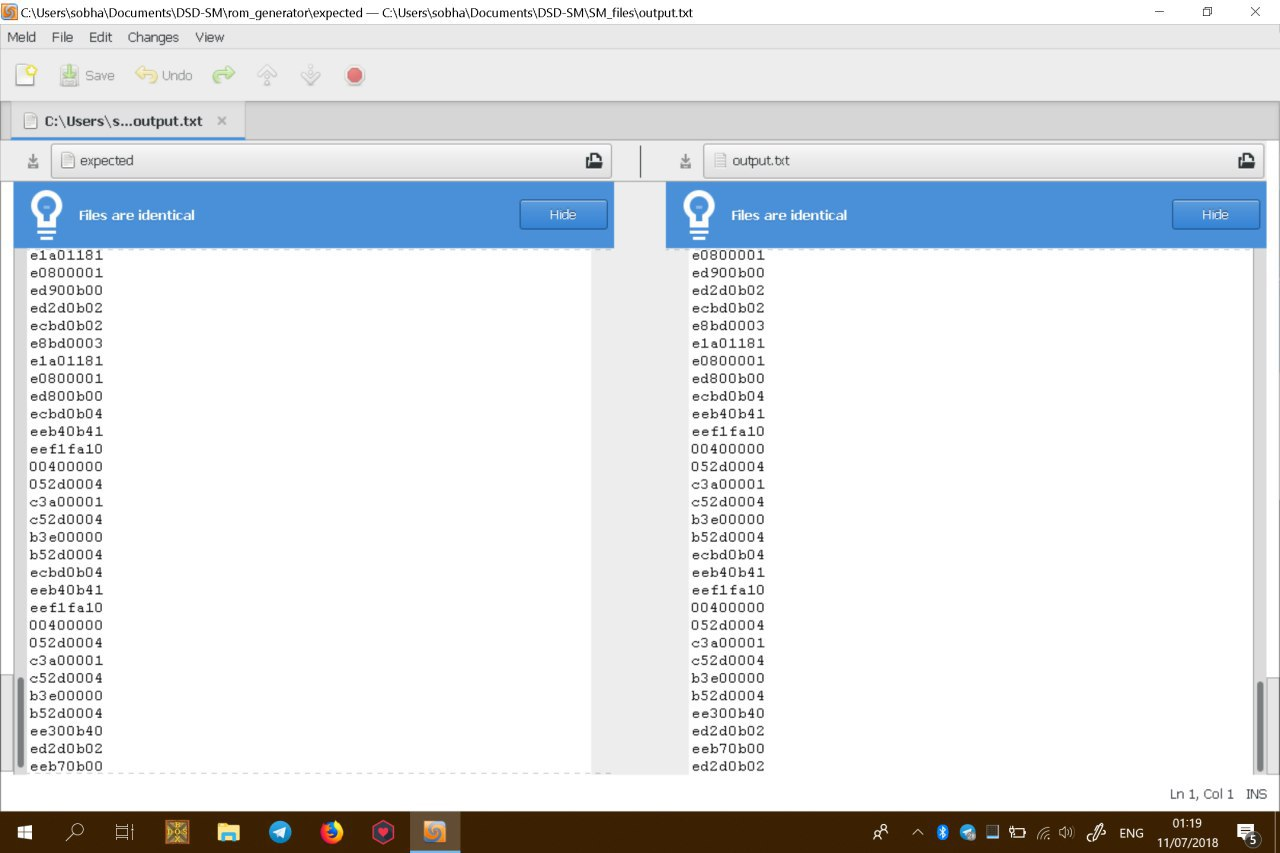
\includegraphics[width=0.8\linewidth]{result}
	\caption{نتیجه‌ی سنتز}
	\label{fig:result}
\end{figure}
